\documentclass[serif]{beamer}\usepackage[]{graphicx}\usepackage[]{color}
%% maxwidth is the original width if it is less than linewidth
%% otherwise use linewidth (to make sure the graphics do not exceed the margin)
\makeatletter
\def\maxwidth{ %
  \ifdim\Gin@nat@width>\linewidth
    \linewidth
  \else
    \Gin@nat@width
  \fi
}
\makeatother

\definecolor{fgcolor}{rgb}{0.345, 0.345, 0.345}
\newcommand{\hlnum}[1]{\textcolor[rgb]{0.686,0.059,0.569}{#1}}%
\newcommand{\hlstr}[1]{\textcolor[rgb]{0.192,0.494,0.8}{#1}}%
\newcommand{\hlcom}[1]{\textcolor[rgb]{0.678,0.584,0.686}{\textit{#1}}}%
\newcommand{\hlopt}[1]{\textcolor[rgb]{0,0,0}{#1}}%
\newcommand{\hlstd}[1]{\textcolor[rgb]{0.345,0.345,0.345}{#1}}%
\newcommand{\hlkwa}[1]{\textcolor[rgb]{0.161,0.373,0.58}{\textbf{#1}}}%
\newcommand{\hlkwb}[1]{\textcolor[rgb]{0.69,0.353,0.396}{#1}}%
\newcommand{\hlkwc}[1]{\textcolor[rgb]{0.333,0.667,0.333}{#1}}%
\newcommand{\hlkwd}[1]{\textcolor[rgb]{0.737,0.353,0.396}{\textbf{#1}}}%
\let\hlipl\hlkwb

\usepackage{framed}
\makeatletter
\newenvironment{kframe}{%
 \def\at@end@of@kframe{}%
 \ifinner\ifhmode%
  \def\at@end@of@kframe{\end{minipage}}%
  \begin{minipage}{\columnwidth}%
 \fi\fi%
 \def\FrameCommand##1{\hskip\@totalleftmargin \hskip-\fboxsep
 \colorbox{shadecolor}{##1}\hskip-\fboxsep
     % There is no \\@totalrightmargin, so:
     \hskip-\linewidth \hskip-\@totalleftmargin \hskip\columnwidth}%
 \MakeFramed {\advance\hsize-\width
   \@totalleftmargin\z@ \linewidth\hsize
   \@setminipage}}%
 {\par\unskip\endMakeFramed%
 \at@end@of@kframe}
\makeatother

\definecolor{shadecolor}{rgb}{.97, .97, .97}
\definecolor{messagecolor}{rgb}{0, 0, 0}
\definecolor{warningcolor}{rgb}{1, 0, 1}
\definecolor{errorcolor}{rgb}{1, 0, 0}
\newenvironment{knitrout}{}{} % an empty environment to be redefined in TeX

\usepackage{alltt}
\usetheme{Boadilla}
\usepackage{graphicx}
\usepackage[final]{animate}
\usepackage{breqn}
\usepackage{xcolor}
\usepackage{booktabs}
\usepackage{tikz}
\usetikzlibrary{decorations.pathreplacing}
\usetikzlibrary{shapes,arrows,positioning,shadows}
\usepackage{subfig}
\usepackage{pgf}
\usepackage{caption}

% change format of enumerated lists
\setbeamertemplate{enumerate items}[default]
\setbeamertemplate{navigation symbols}{}

% macros
\newcommand{\emtxt}[1]{\textbf{\textit{{\color{mypal4} #1}}}}

% change font size for figure captions
\setbeamerfont{caption}{size=\scriptsize}

% custom colors
\definecolor{mypal1}{HTML}{F0F9E8}\definecolor{mypal2}{HTML}{BAE4BC}\definecolor{mypal3}{HTML}{7BCCC4}\definecolor{mypal4}{HTML}{43A2CA}\definecolor{mypal5}{HTML}{0868AC}

\tikzstyle{decision} = [diamond, draw, text width=6em, text badly centered, inner sep = 2pt, top color=white, bottom color=mypal3, drop shadow]
\tikzstyle{block} = [rectangle, draw, text width=10em, text centered, rounded corners, minimum height=3em, minimum width=8em, top color = white, bottom color=mypal4,  drop shadow]
\tikzstyle{declare} = [rectangle, draw, text width=10em, text centered, minimum height=3em, minimum width=8em, top color = white, bottom color=mypal5,  drop shadow]

% knitr setup


% dependent data


% get online bib file


% part of figure used on title page


\setbeamercolor{title}{fg=mypal5} % main title
\setbeamercolor{frametitle}{fg=mypal4, bg=mypal2} % frame titles
\setbeamercolor{structure}{fg=mypal4} % bottom banner
\setbeamercolor{normal text}{fg=mypal5}
\usebackgroundtemplate{
\includegraphics[height=\paperheight,width=\paperwidth]{fig/back_tmp.pdf}}
\IfFileExists{upquote.sty}{\usepackage{upquote}}{}
\begin{document}

\title[Seagrass light requirements]{\textbf{Quantifying seagrass light requirements using an algorithm to spatially resolve depth of colonization}}
\author[M. Beck, J. Hagy, C. Le]{Marcus W. Beck, James D. Hagy III, Chengfeng Le}

\institute[USEPA]{USEPA National Health and Environmental Effects Research Laboratory, Gulf Ecology Division, \href{mailto:beck.marcus@epa.gov}{beck.marcus@epa.gov}, Phone: 8509342480}

\date{Nov. 4, 2016}

\titlegraphic{
\begin{minipage}{0.4\textwidth}
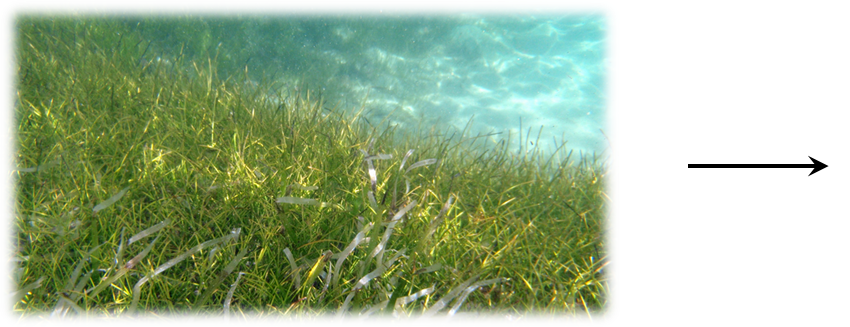
\includegraphics[width=\linewidth]{fig/titlegraphic.png}
\end{minipage}
\begin{minipage}{0.27\linewidth}
\vspace{0.05in}
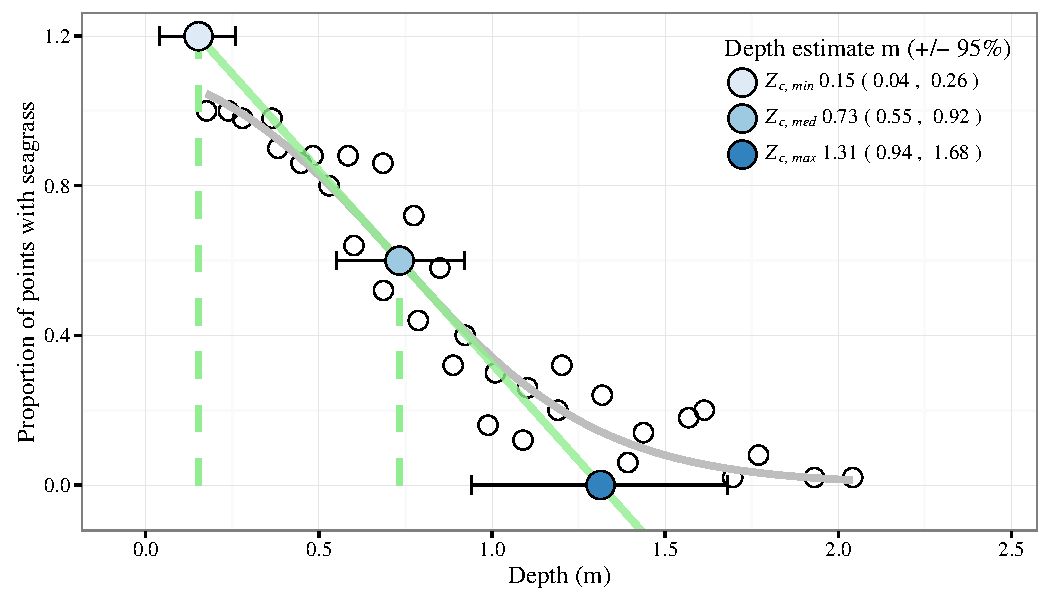
\includegraphics[width=\linewidth]{fig/doc_title.pdf}
\end{minipage}
}

%%%%%%
\begin{frame}[shrink]
\vspace{0.2in}
\titlepage
\end{frame}

\section{Background}

%%%%%%
\begin{frame}{$\vcenter{\hbox{
\includegraphics[width=0.05\paperwidth]{fig/epa_logo.png}}}$\hspace{0.07in}\textbf{Seagrasses and water quality}}
\begin{center}
Seagrasses are beneficial - healthy seagrass, healthy estuary {\tiny \cite{Williams01,Hughes09}}
\end{center}
\centerline{\fbox{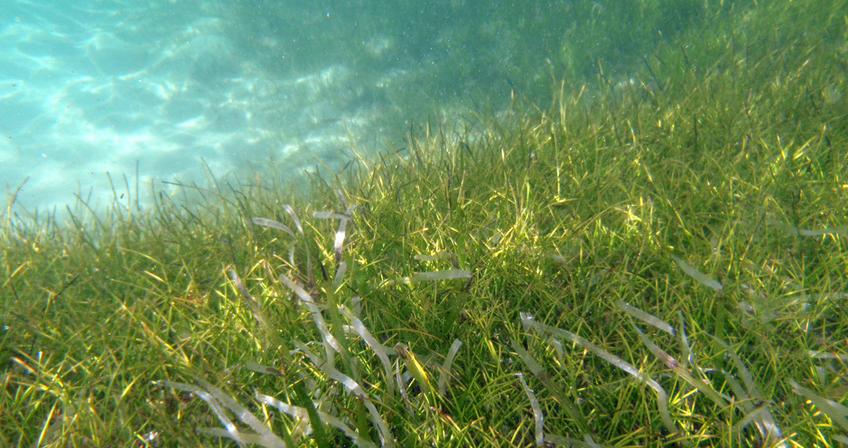
\includegraphics[width = 0.65\textwidth]{fig/sg_pic.png}}}
\begin{center}
Seagrasses are sentinels of water quality {\tiny \cite{Duarte95,Short96}}
\end{center}
\vfill
\tiny
\hfill \href{https://www.flickr.com/photos/swimvixen2/3581613875/in/photostream/}{flickr.com/photos/swimvixen2}
\end{frame}

%%%%%%
\begin{frame}{$\vcenter{\hbox{
\includegraphics[width=0.05\paperwidth]{fig/epa_logo.png}}}$\hspace{0.07in}\textbf{Research challenges and study objective}}
\onslide<+->
The maximum depth of colonization is a useful proxy of eutrophication {\tiny \cite{Kenworthy96,Choice14}} \\~\\
Often used as a basis for establishing nutrient criteria {\tiny \cite{Steward07}}\\~\\
\onslide<+->
\emtxt{Problem 1:} No consensus on the best way to measure depth of colonization \\~\\
\emtxt{Problem 2:} Plenty of data are available but standardized techniques have not been developed \\~\\
\onslide<+->
\begin{block}{Study objective}
Develop and apply an algorithm that uses geospatial data to describe relationships between seagrass depth limits, water clarity, and light requirements \scriptsize [Beck, Hagy, Le, in review]
\end{block}
\end{frame}

%%%%%%
\begin{frame}{$\vcenter{\hbox{
\includegraphics[width=0.05\paperwidth]{fig/epa_logo.png}}}$\hspace{0.07in}\textbf{Estimating seagrass depth of colonization}}
\onslide<+->
\emtxt{Existing geospatial datasets} - coastal segments, seagrass areal coverage, bathymetry
\begin{columns}[T]
\begin{column}{0.5\textwidth}
\begin{knitrout}
\definecolor{shadecolor}{rgb}{0.969, 0.969, 0.969}\color{fgcolor}

{\centering 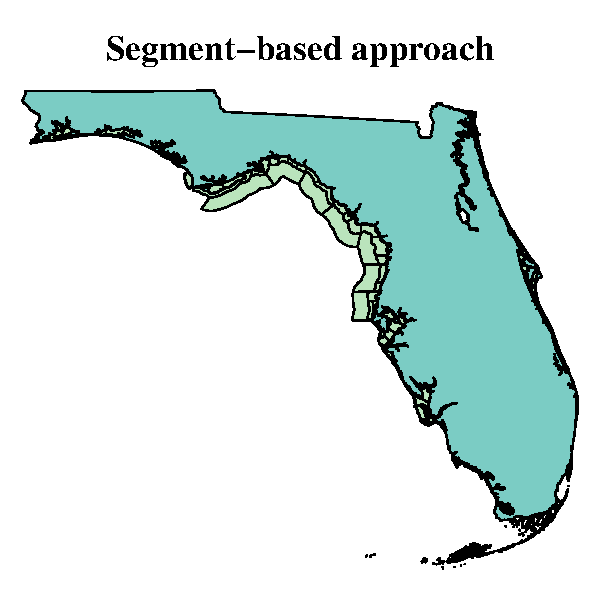
\includegraphics[width=\maxwidth]{fig//segmap-1} 

}



\end{knitrout}
\end{column}
\begin{column}{0.45\textwidth}
\centerline{\fbox{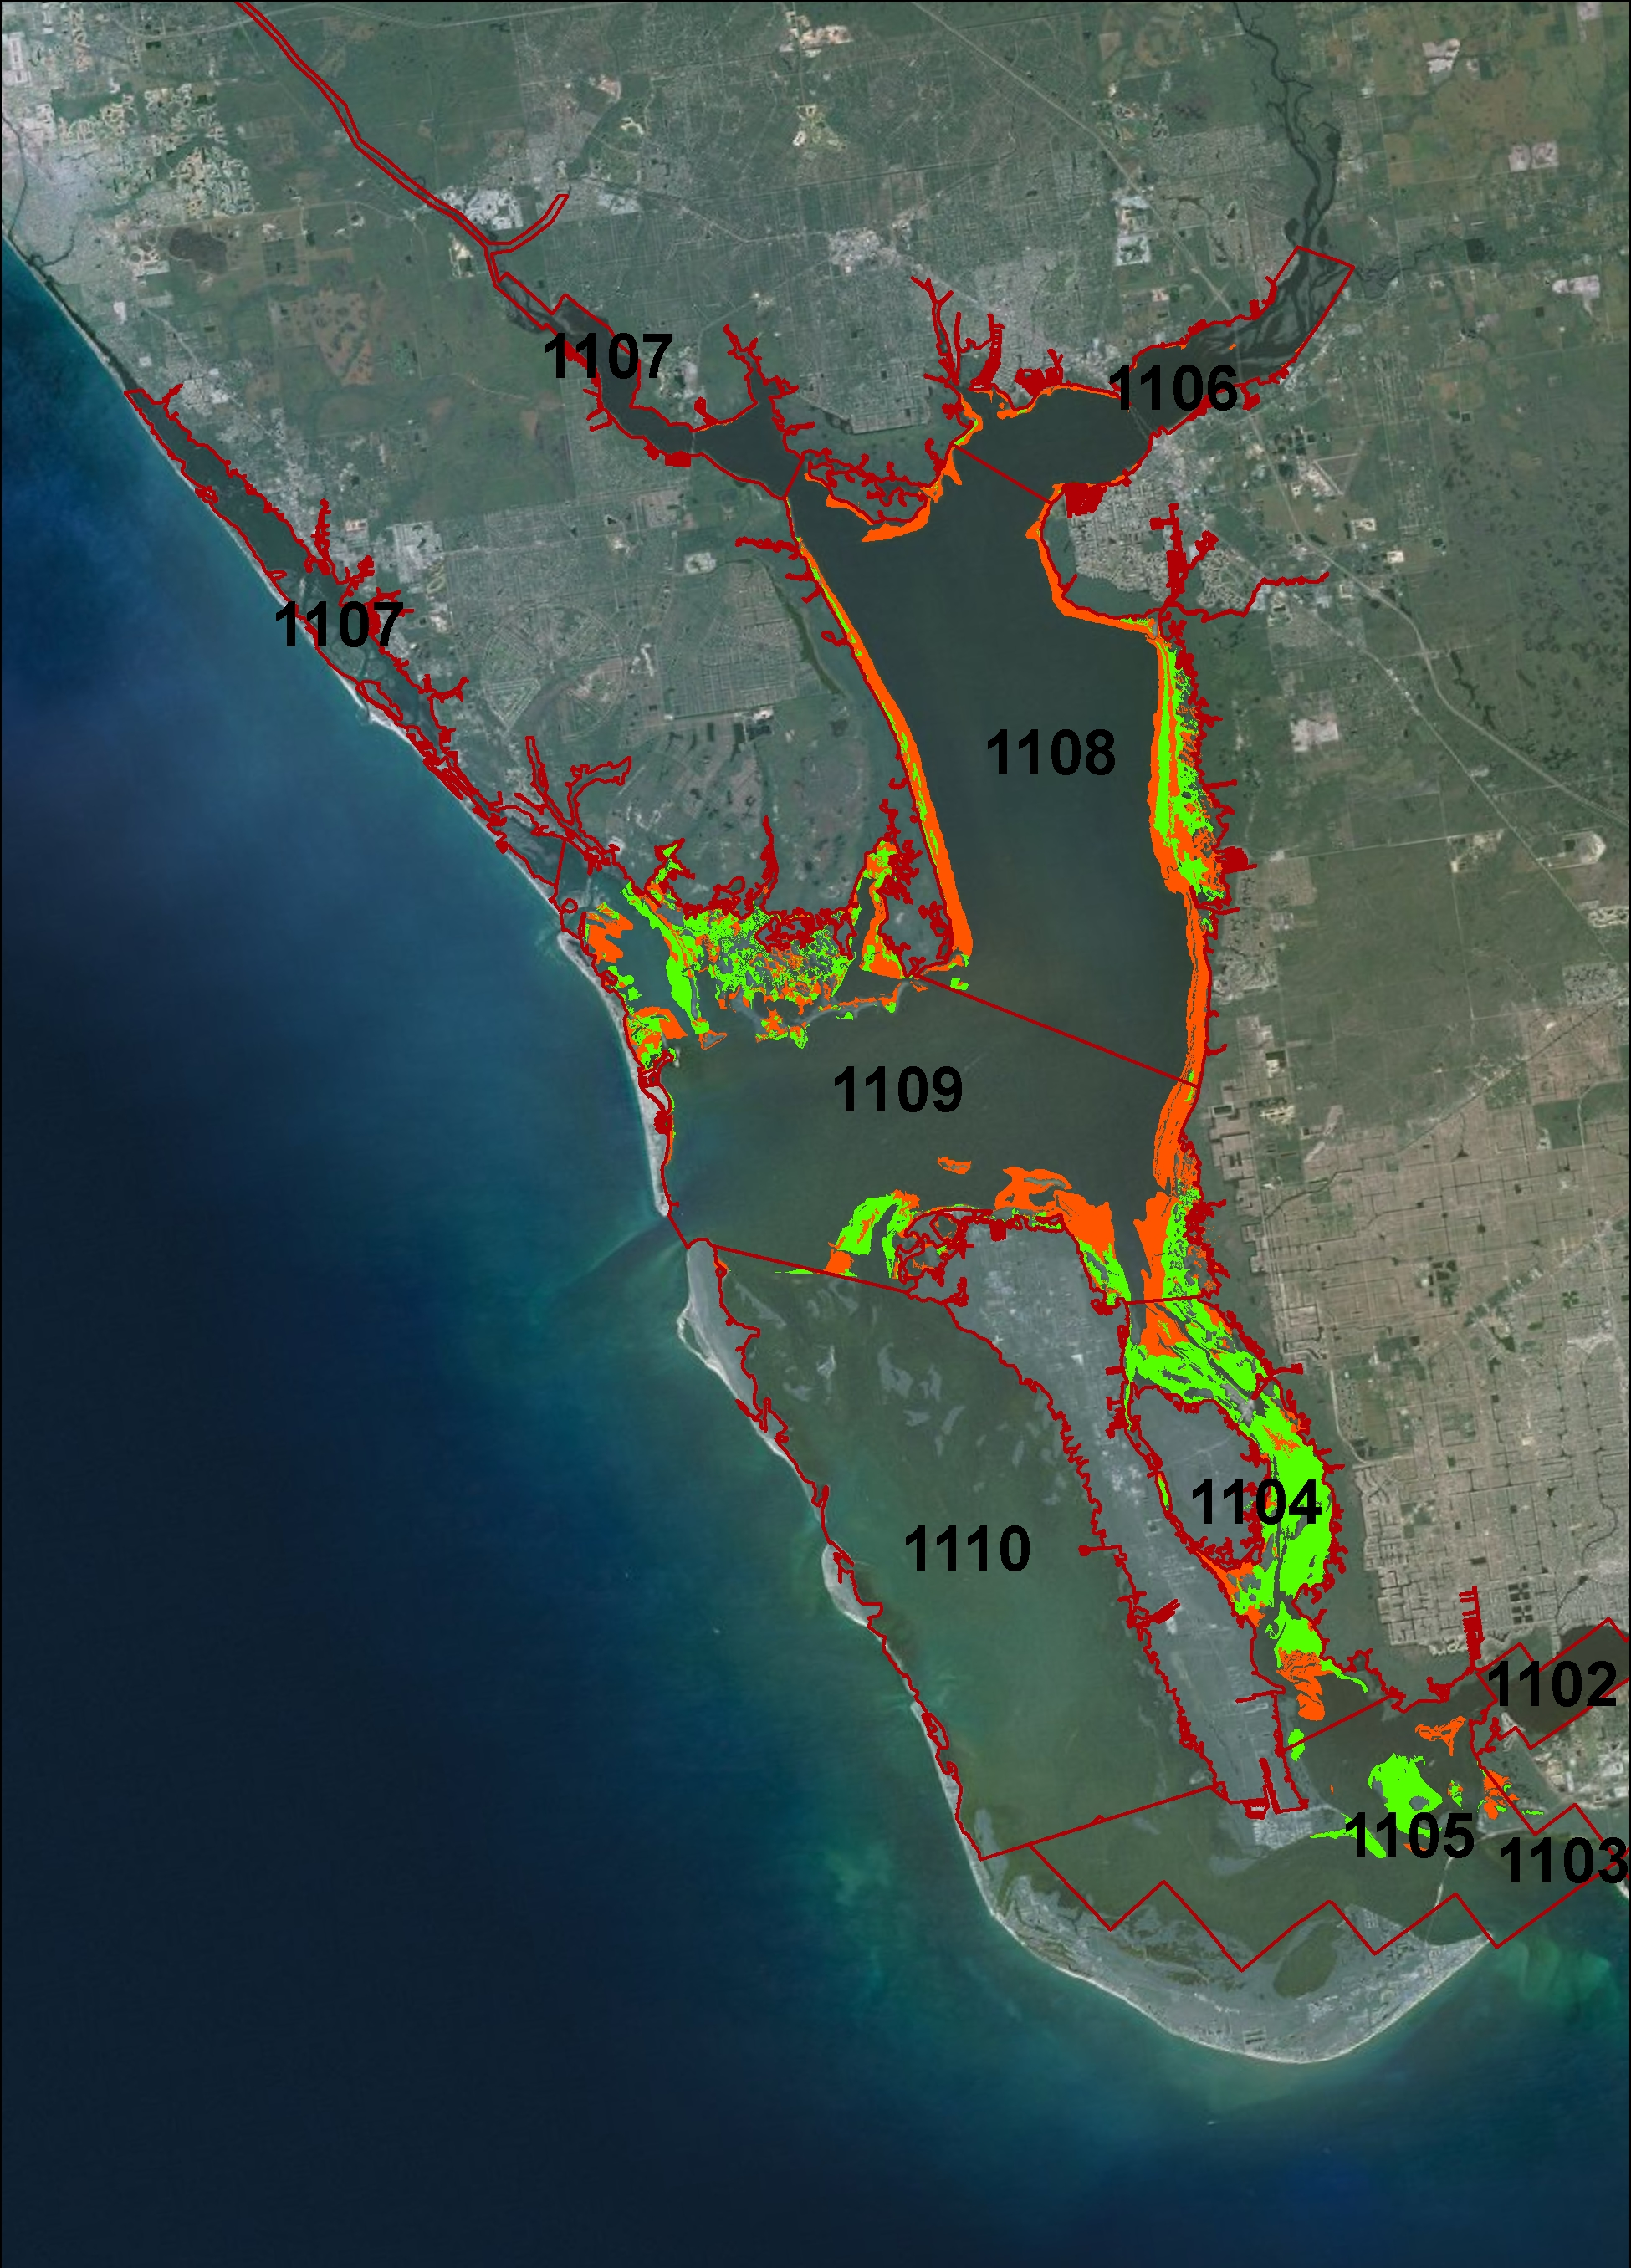
\includegraphics[width = 0.8\textwidth]{fig/Charlotte_Estuary_Segments.jpg}}}
\end{column}
\end{columns}
\end{frame}

%%%%%%
\begin{frame}{$\vcenter{\hbox{
\includegraphics[width=0.05\paperwidth]{fig/epa_logo.png}}}$\hspace{0.07in}\textbf{Estimating seagrass depth of colonization}}
\onslide<+->
How can we estimate depth of colonization? \\~\\
\begin{columns}[T]
\onslide<+->
\begin{column}{0.32\textwidth}
\emtxt{1.} Pick a segment\\~\\
\centerline{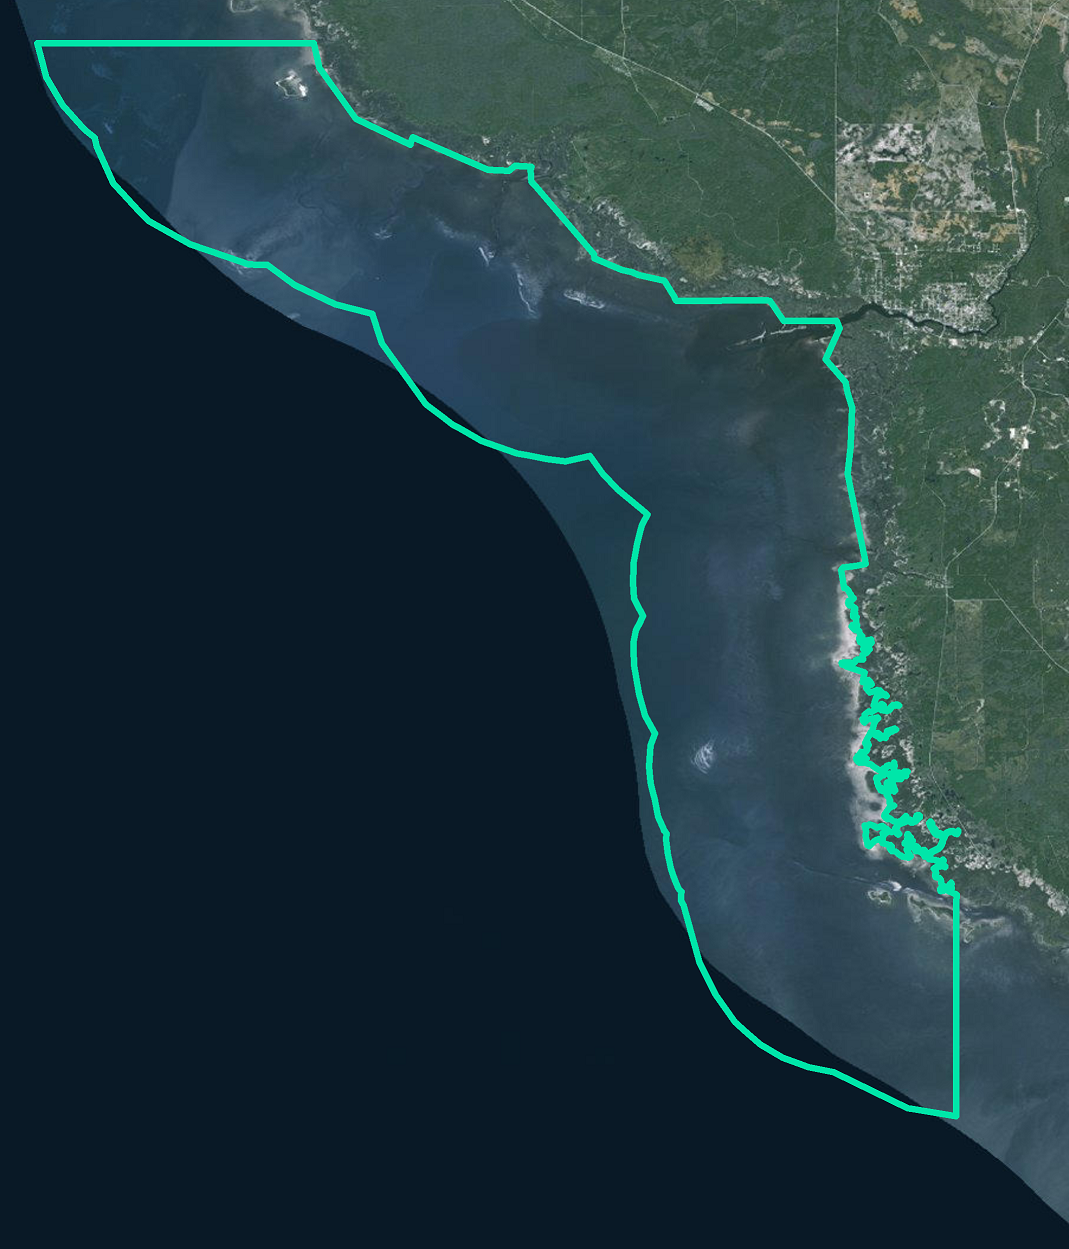
\includegraphics[width = 0.9\textwidth]{fig/map820.png}}
\end{column}
\onslide<+->
\begin{column}{0.32\textwidth}
\emtxt{2.} Get seagrass area \\~\\
\begin{knitrout}
\definecolor{shadecolor}{rgb}{0.969, 0.969, 0.969}\color{fgcolor}

{\centering 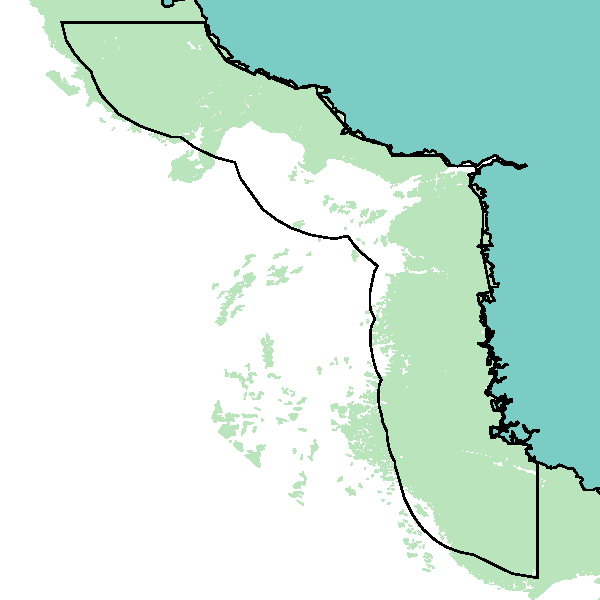
\includegraphics[width=\maxwidth]{fig//segsg-1} 

}



\end{knitrout}
\end{column}
\onslide<+->
\begin{column}{0.32\textwidth}
\emtxt{3.} Get depth points\\~\\
\begin{knitrout}
\definecolor{shadecolor}{rgb}{0.969, 0.969, 0.969}\color{fgcolor}

{\centering 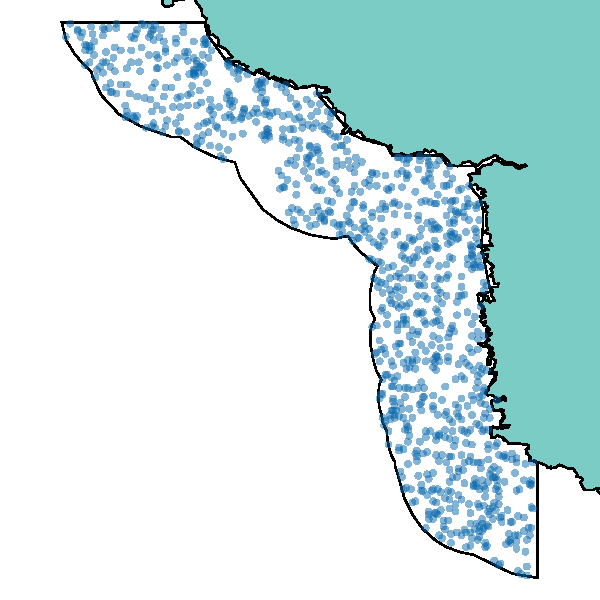
\includegraphics[width=\maxwidth]{fig//segpt-1} 

}



\end{knitrout}
\end{column}
\end{columns}
\vspace{0.15in}
\onslide<+->
\emtxt{4.} Match depth points with seagrass presence/absence...
\end{frame}



%%%%%%
\begin{frame}{$\vcenter{\hbox{
\includegraphics[width=0.05\paperwidth]{fig/epa_logo.png}}}$\hspace{0.07in}\textbf{Estimating seagrass depth of colonization}}
\emtxt{5.} Plot the distribution of seagrass by increasing depth \\~\\
\includegraphics<1>[width = \textwidth, page = 1]{fig/doc_ex.pdf}
\includegraphics<2>[width = \textwidth, page = 2]{fig/doc_ex.pdf}
\includegraphics<3>[width = \textwidth, page = 3]{fig/doc_ex.pdf}
\end{frame}

%%%%%%
\begin{frame}{$\vcenter{\hbox{
\includegraphics[width=0.05\paperwidth]{fig/epa_logo.png}}}$\hspace{0.07in}\textbf{SEstimating seagrass depth of colonization}}
\onslide<+->
The estimate depends on the spatial context...\\~\\
\begin{columns}[T]
\onslide<+->
\begin{column}{0.45\textwidth}
\begin{knitrout}
\definecolor{shadecolor}{rgb}{0.969, 0.969, 0.969}\color{fgcolor}

{\centering 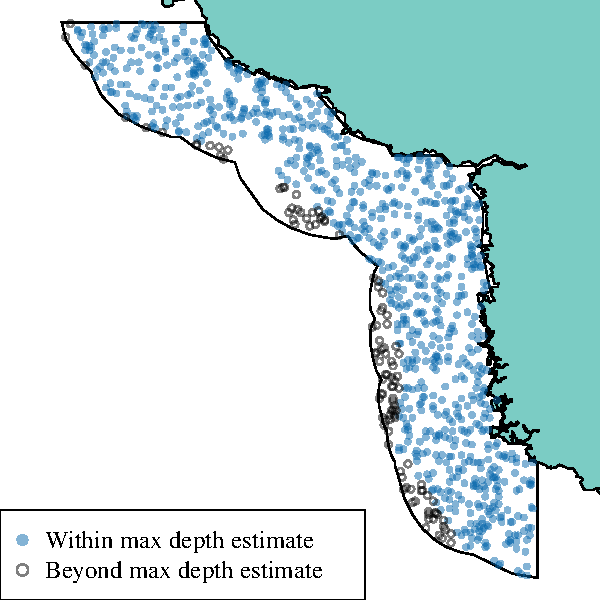
\includegraphics[width=\maxwidth]{fig//docfail1-1} 

}



\end{knitrout}
\end{column}
\onslide<+->
\begin{column}{0.45\textwidth}
\begin{knitrout}
\definecolor{shadecolor}{rgb}{0.969, 0.969, 0.969}\color{fgcolor}

{\centering 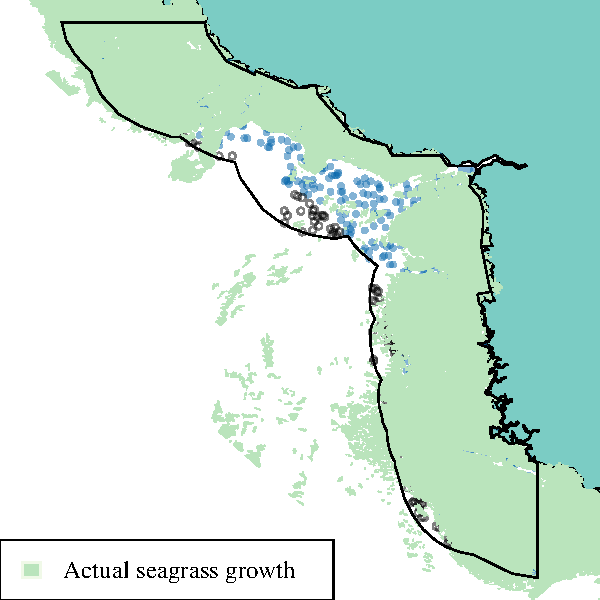
\includegraphics[width=\maxwidth]{fig//docfail2-1} 

}



\end{knitrout}
\end{column}
\end{columns}
\end{frame}


%%%%%%
\begin{frame}{$\vcenter{\hbox{
\includegraphics[width=0.05\paperwidth]{fig/epa_logo.png}}}$\hspace{0.07in}\textbf{Estimating seagrass depth of colonization}}
The estimate depends on the spatial context...
\begin{center}
\animategraphics[controls,width=\linewidth,trim = 15mm 2mm 0mm 0mm]{6}{fig/radred}{}{} %frame rate is 12 per/sec
\end{center}
\end{frame}



%%%%%%
\begin{frame}{$\vcenter{\hbox{
\includegraphics[width=0.05\paperwidth]{fig/epa_logo.png}}}$\hspace{0.07in}\textbf{Estimating seagrass depth of colonization}}
The estimate depends on the spatial context...
\begin{center}
\animategraphics[controls,width=0.95\linewidth]{6}{fig/radred2}{}{} %frame rate is 12 per/sec
\end{center}
\end{frame}



%%%%%%
\begin{frame}{$\vcenter{\hbox{
\includegraphics[width=0.05\paperwidth]{fig/epa_logo.png}}}$\hspace{0.07in}\textbf{Estimating seagrass depth of colonization}}
The algorithm was applied to entire estuaries with appropriate data \\~\\
\begin{columns}
\begin{column}{0.3\textwidth}
\emtxt{Boundaries}
\begin{center}
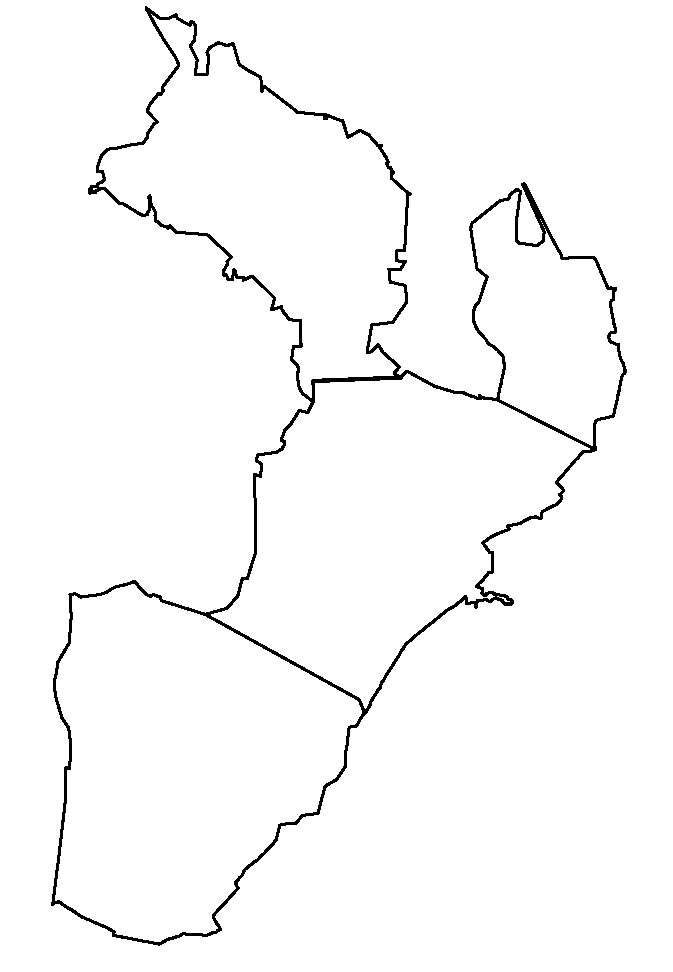
\includegraphics[width = \textwidth]{fig/tb_seg.pdf}
\end{center}
\end{column}
\begin{column}{0.3\textwidth}
\emtxt{Depth}
\begin{center}
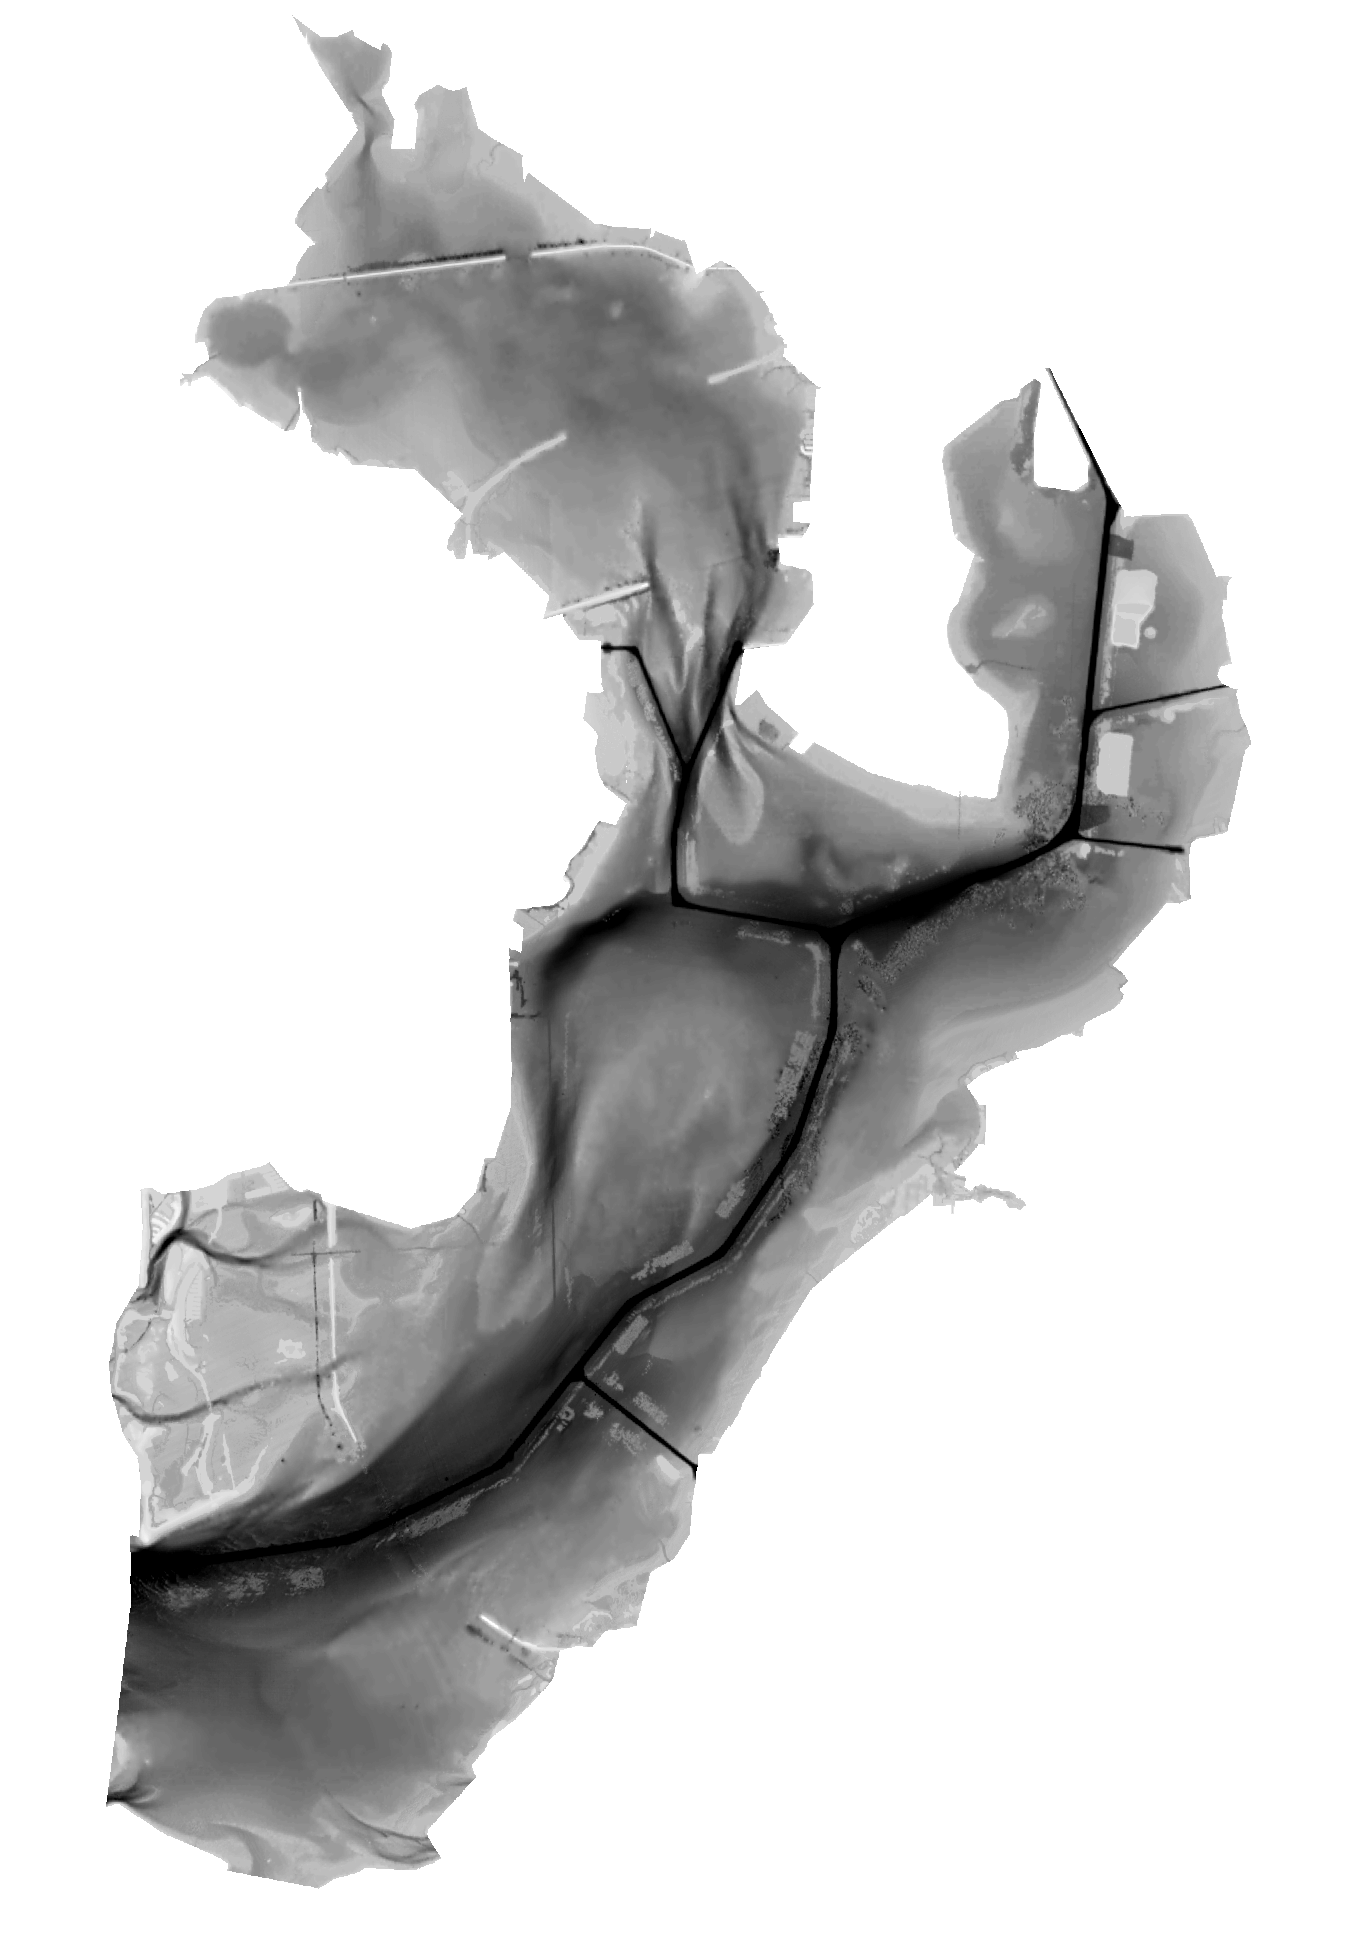
\includegraphics[width = \textwidth]{fig/tb_dem.png}
\end{center}
\end{column}
\begin{column}{0.3\textwidth}
\emtxt{Seagrass}
\begin{center}
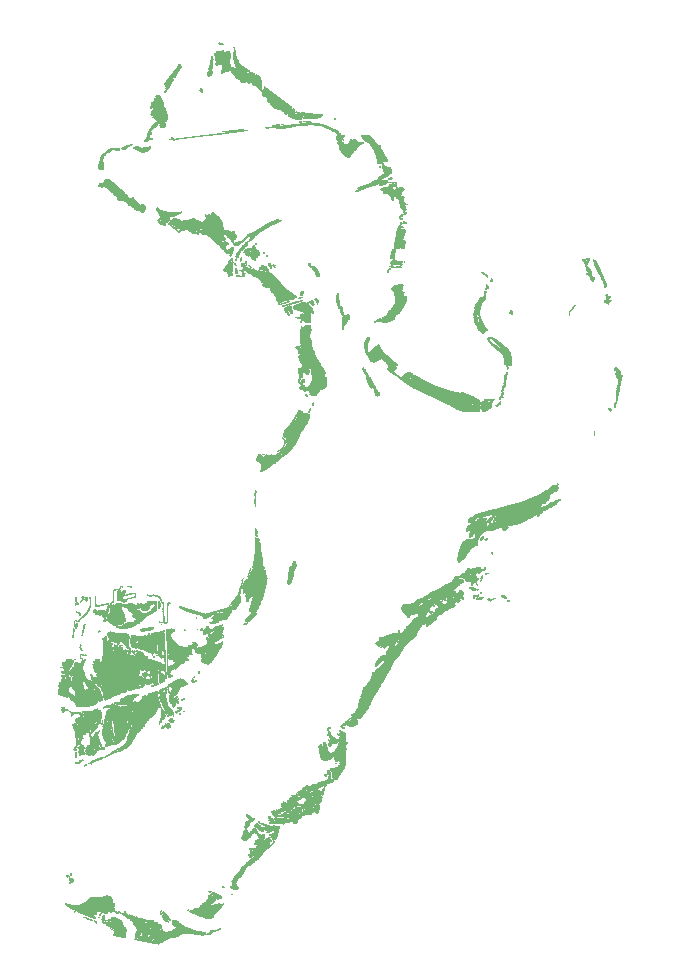
\includegraphics[width = \textwidth]{fig/tb_sgr.pdf}
\end{center}
\end{column}
\end{columns}
\end{frame}

% tb summ


%%%%%%
\begin{frame}[t]{$\vcenter{\hbox{
\includegraphics[width=0.05\paperwidth]{fig/epa_logo.png}}}$\hspace{0.07in}\textbf{Linking estimates to light requirements}}
Tampa Bay summary: \\~\\
\centerline{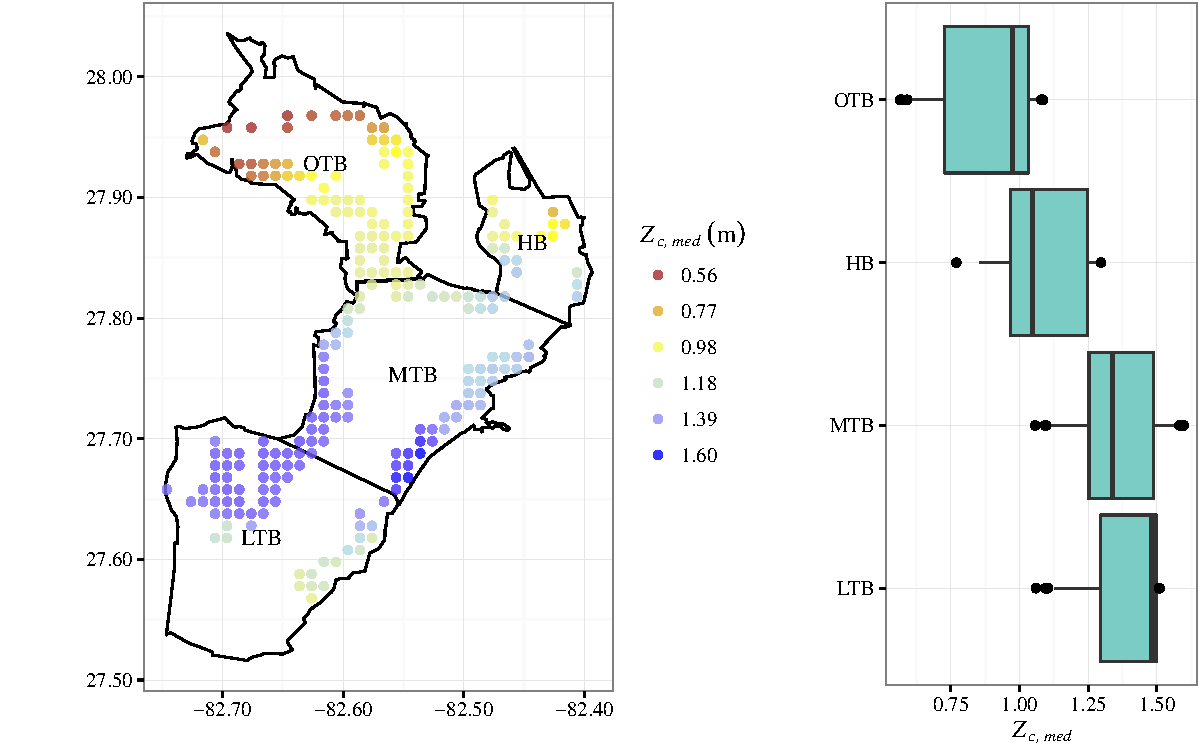
\includegraphics[width = 0.85\textwidth]{fig/tb_summ1.pdf}}
\end{frame}



%%%%%%
\begin{frame}{$\vcenter{\hbox{
\includegraphics[width=0.05\paperwidth]{fig/epa_logo.png}}}$\hspace{0.07in}\textbf{Linking estimates to light requirements}}
\onslide<1->
Can we link depth estimates with water clarity to understand light requirements?
\vspace{-0.2in}
\begin{columns}[t]
\footnotesize
\begin{column}{0.3\textwidth}
\onslide<1->
\begin{center}
\emtxt{Depth of colonization}
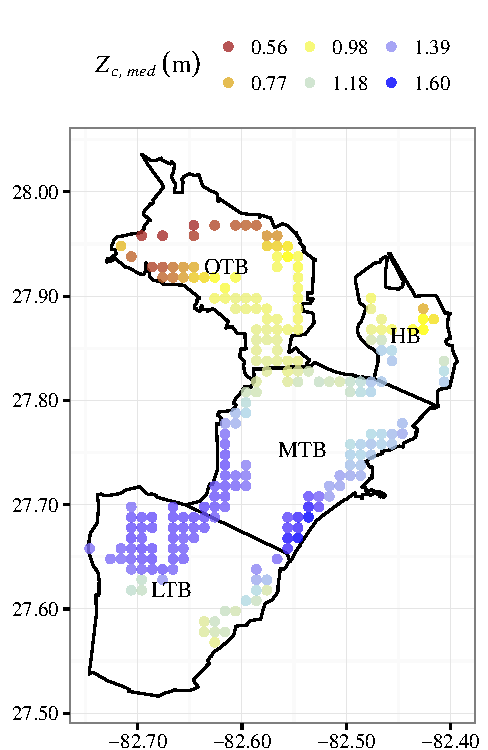
\includegraphics[width = \textwidth]{fig/tb_zcmed.pdf}
\end{center}
\end{column}
\begin{column}{0.64\textwidth}
\onslide<2->
\vspace{0.2in}
\begin{center}
$\%SI = 100 \cdot \frac{I_{z}}{I_{o}} = exp\left(-K_d \cdot Z_{c,med}\right)$ \\~\\
$I_z$: irradiance at depth \\
$I_o$: irradiance at surface \\
$K_d$: light extinction coefficient 
\end{center}
\begin{itemize}
\item Percent surface irradiance at depth as a measure of seagrass light requirements \\~\\
\item Can be used to characterize light regimes that maintain seagrass habitat
\end{itemize}
\end{column}
\end{columns}
\end{frame}

%%%%%%
\begin{frame}{$\vcenter{\hbox{
\includegraphics[width=0.05\paperwidth]{fig/epa_logo.png}}}$\hspace{0.07in}\textbf{Linking estimates to light requirements}}
\onslide<1->
Can we link depth estimates with water clarity to understand light requirements?
\vspace{-0.2in}
\begin{columns}[t]
\footnotesize
\begin{column}{0.3\textwidth}
\begin{center}
\onslide<1->
\emtxt{Depth of colonization}
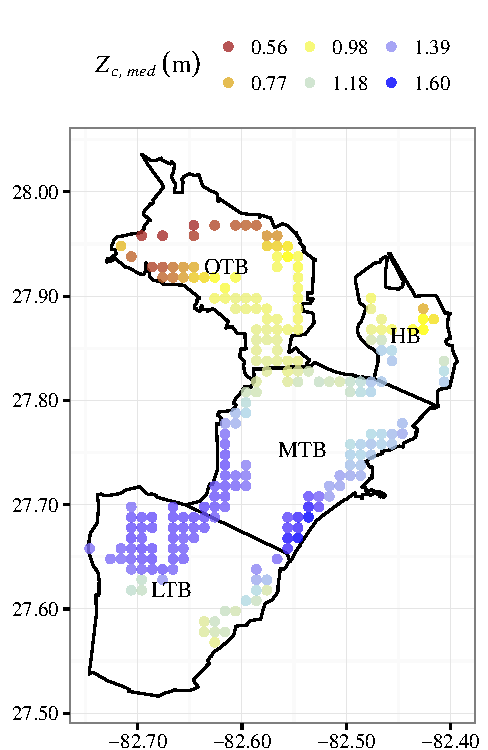
\includegraphics[width = \textwidth]{fig/tb_zcmed.pdf}
\end{center}
\end{column}
\begin{column}{0.3\textwidth}
\begin{center}
\onslide<1->
\emtxt{Water clarity}
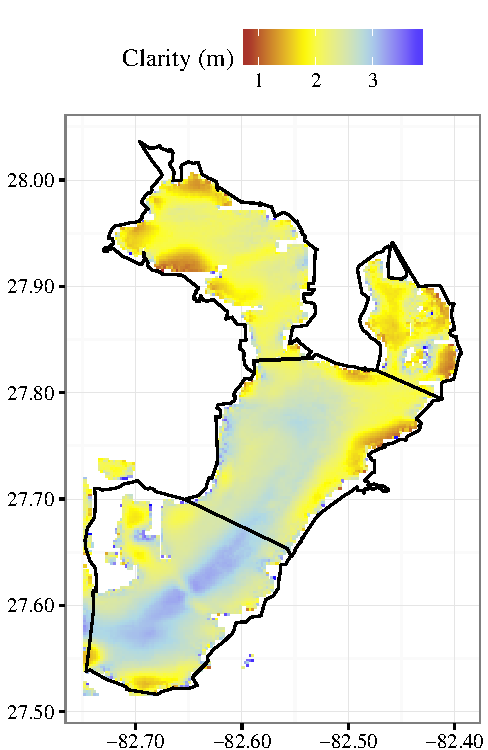
\includegraphics[width = 0.97\textwidth, clip = true, trim = 0mm 0mm 0mm -3mm]{fig/tb_sats.pdf}
\end{center}
\end{column}
\begin{column}{0.3\textwidth}
\begin{center}
\onslide<2->
\emtxt{Light requirements}
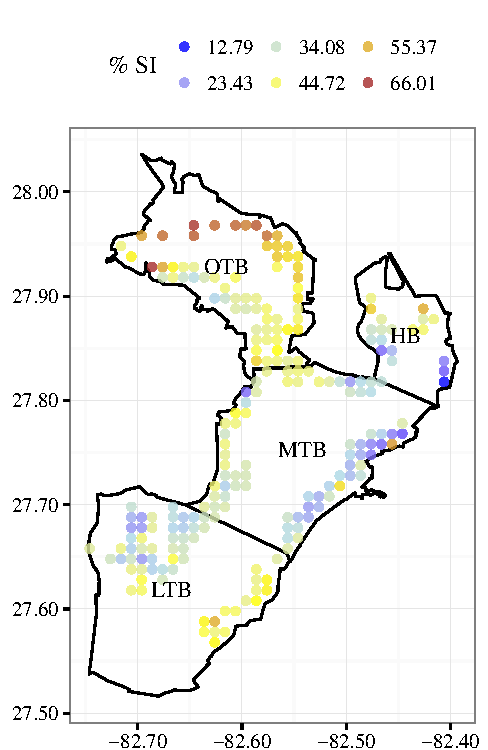
\includegraphics[width = \textwidth]{fig/tb_light.pdf}
\end{center}
\end{column}
\end{columns}
\end{frame}

%%%%%%
\begin{frame}[t]{$\vcenter{\hbox{
\includegraphics[width=0.05\paperwidth]{fig/epa_logo.png}}}$\hspace{0.07in}\textbf{Linking estimates to light requirements}}
Tampa Bay summary: \\~\\
\centerline{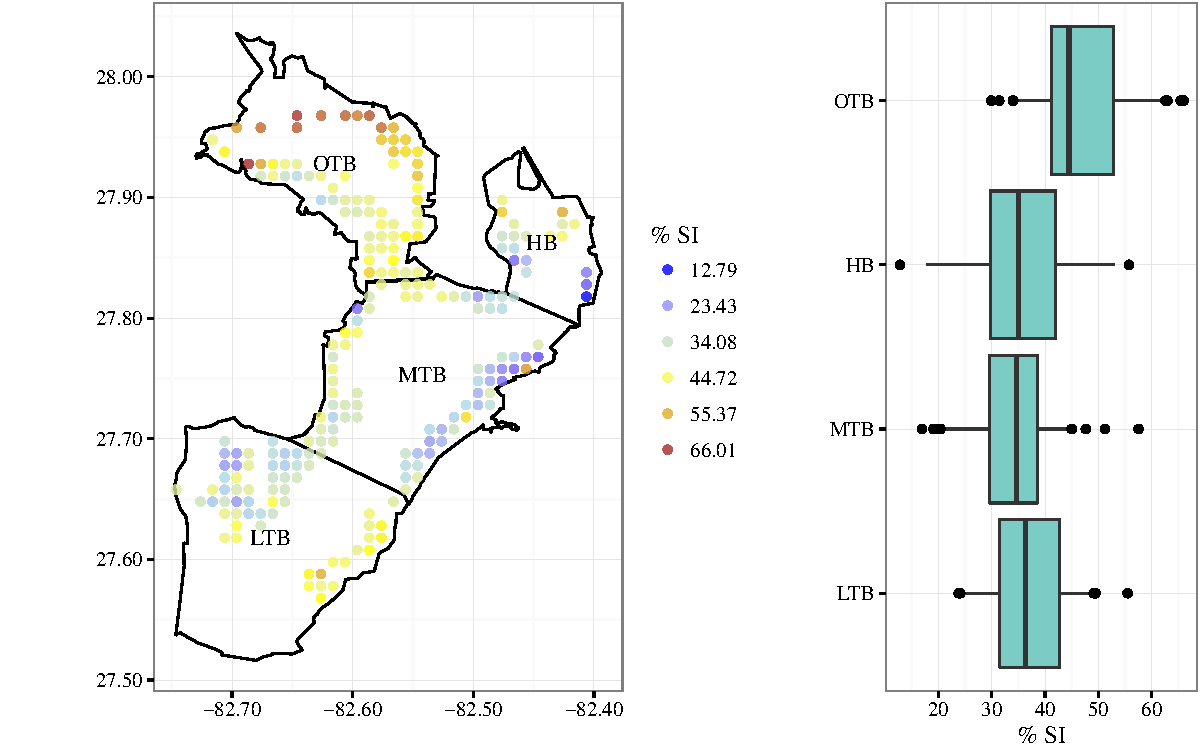
\includegraphics[width = 0.85\textwidth]{fig/tb_summ2.pdf}}
\end{frame}

%%%%%%
\begin{frame}{$\vcenter{\hbox{
\includegraphics[width=0.05\paperwidth]{fig/epa_logo.png}}}$\hspace{0.07in}\textbf{Linking estimates to light requirements}}
\scriptsize
%latex.default(tabzc, file = "", rowlabel = "Segment", caption = cap.val,     colheads = col_heads, cgroup = c("", "$\\mathbf Z_{c,\\,med}$"),     n.cgroup = c(1, 4), caption.loc = "top", rowname = rows)%
\begin{table}[!tbp]
\caption{Summary of median depth of colonization ($Z_{c,\,med}$, m) for Tampa Bay and bay segments.\label{tabzc}} 
\begin{center}
\begin{tabular}{llcllll}
\hline\hline
\multicolumn{1}{l}{\bfseries Segment}&\multicolumn{1}{c}{\bfseries }&\multicolumn{1}{c}{\bfseries }&\multicolumn{4}{c}{\bfseries $\mathbf Z_{c,\,med}$}\tabularnewline
\cline{4-7}
\multicolumn{1}{l}{}&\multicolumn{1}{c}{$n$}&\multicolumn{1}{c}{}&\multicolumn{1}{c}{Mean}&\multicolumn{1}{c}{St. Err.}&\multicolumn{1}{c}{Min}&\multicolumn{1}{c}{Max}\tabularnewline
\hline
\textbf{Tampa Bay}&218&&1.2\textsuperscript{}&0.1&0.6&1.6\tabularnewline
\hspace{0.02in} HB&20&&1.1\textsuperscript{ab}&0.2&0.8&1.3\tabularnewline
\hspace{0.02in} LTB&60&&1.3\textsuperscript{b}&0.1&1.1&1.5\tabularnewline
\hspace{0.02in} MTB&74&&1.4\textsuperscript{b}&0.1&1.1&1.6\tabularnewline
\hspace{0.02in} OTB&64&&0.8\textsuperscript{a}&0.2&0.6&1.1\tabularnewline
\hline
\end{tabular}\end{center}

\end{table}
%latex.default(tablt, file = "", rowlabel = "Segment", caption = cap.val,     colheads = col_heads, cgroup = c("", "{\\bf \\% light}"),     n.cgroup = c(1, 4), caption.loc = "top", rowname = rows)%
\begin{table}[!tbp]
\caption{Summary of light requirements (\%) for Tampa Bay and bay segments.\label{tablt}} 
\begin{center}
\begin{tabular}{llcllll}
\hline\hline
\multicolumn{1}{l}{\bfseries Segment}&\multicolumn{1}{c}{\bfseries }&\multicolumn{1}{c}{\bfseries }&\multicolumn{4}{c}{\bfseries {\bf \% light}}\tabularnewline
\cline{4-7}
\multicolumn{1}{l}{}&\multicolumn{1}{c}{$n$}&\multicolumn{1}{c}{}&\multicolumn{1}{c}{Mean}&\multicolumn{1}{c}{St. Err.}&\multicolumn{1}{c}{Min}&\multicolumn{1}{c}{Max}\tabularnewline
\hline
\textbf{Tampa Bay}&218&&41\textsuperscript{}&2.5&13&66\tabularnewline
\hspace{0.02in} HB&20&&34.1&11.2&12.8&55.7\tabularnewline
\hspace{0.02in} LTB&60&&40.0& 7.5&23.8&55.5\tabularnewline
\hspace{0.02in} MTB&74&&36.1& 7.6&17.0&57.5\tabularnewline
\hspace{0.02in} OTB&64&&48.9& 8.7&29.9&66.0\tabularnewline
\hline
\end{tabular}\end{center}

\end{table}

\end{frame}

%%%%%%
\begin{frame}{$\vcenter{\hbox{
\includegraphics[width=0.05\paperwidth]{fig/epa_logo.png}}}$\hspace{0.07in}\textbf{Conclusions}}
\onslide<1->
Benefits of the approach: \\~\\
\begin{itemize}
\onslide<1-> 
\item Better characterization of \emtxt{spatial patterns} - 20\% light requirements may not be sufficient for all \\~\\
\onslide<2-> 
\item The spatial unit for any estimate of seagrass growth limit is \emtxt{problem-specific} - a `compliance-point' approach \\~\\
\onslide<3-> 
\item Increased understanding of seagrass growth patterns can lead to \emtxt{testable hypotheses}
\end{itemize}
\vspace{0.07in}
\onslide<1-> 
\centerline{\fbox{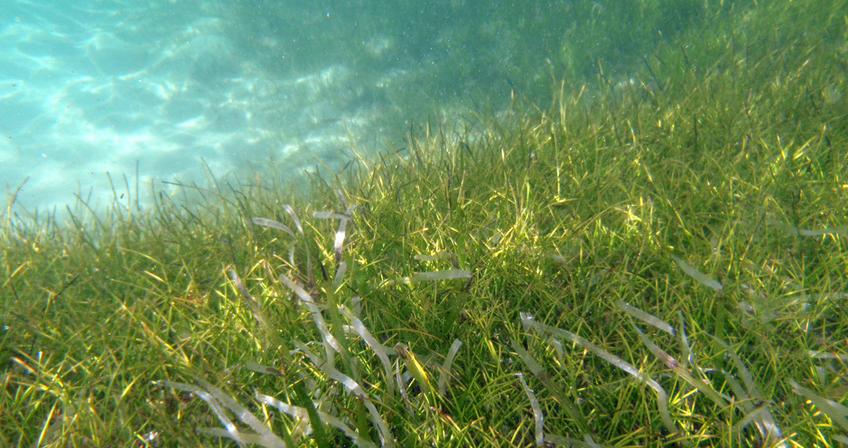
\includegraphics[width = 0.31\textwidth]{fig/sg_pic.png}}}
\end{frame}

%%%%%%
\begin{frame}
\emtxt{Acknowledgments:}\\~\\
\begin{columns}
\begin{column}{0.55\textwidth}
{\footnotesize
Research staff and employees at USEPA Gulf Ecology Division \\~\\
Field staff and data managers at Hillsborough County Environmental Protection Commission, Tampa Bay Estuary Program\\~\\
Peter Tango for reviewing a manuscript draft
}
\end{column}
\begin{column}{0.4\textwidth}
\vspace{-0.2in}
\begin{center}
{\tiny
Online app \href{https://beckmw.shinyapps.io/sg_depth/}{https://beckmw.shinyapps.io/sg\_depth/}\\~\\
}
\centerline{\fbox{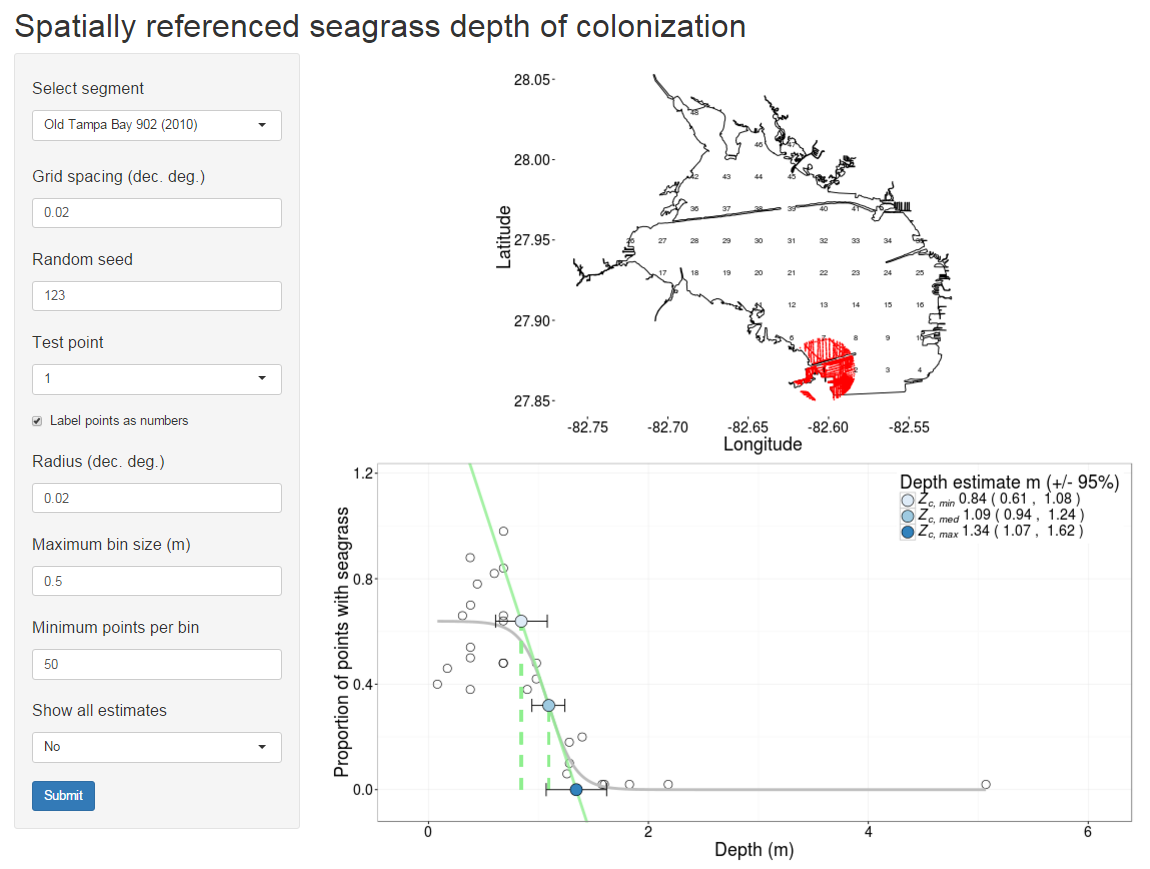
\includegraphics[width=0.85\linewidth]{fig/app.PNG}}}
\end{center}
\end{column}
\end{columns}
\vfill
\emtxt{Funding sources and contact:}\\~\\
\begin{columns}
\begin{column}{0.5\textwidth}
\centerline{
\includegraphics[width=0.4\linewidth]{fig/epa_logo.png}}
\end{column}
\begin{column}{0.5\textwidth}
\scriptsize
\href{mailto:beck.marcus@epa.gov}{beck.marcus@epa.gov} \\~\\
Phone: 8509342480 \\~\\
Github: \href{https://github.com/fawda123/}{github.com/fawda123/} \\~\\
Blog: \href{http://beckmw.wordpress.com/}{beckmw.wordpress.com/}
\end{column}
\end{columns}
\vspace{0.2in}
\end{frame}

%%%%%%
\section{References}
\begin{frame}[t]{\textbf{References}}
\tiny
\setbeamertemplate{bibliography item}{}
\bibliographystyle{apalike_mine}
\bibliography{refs}
\end{frame}

\end{document}
